\documentclass[english,hidelinks, 11 pt, class=report,crop=false]{standalone}
\usepackage[T1]{fontenc}
%\usepackage[utf8]{inputenc}
\usepackage{lmodern} % load a font with all the characters
\usepackage{geometry}
\geometry{verbose,paperwidth=16.1 cm, paperheight=24 cm, inner=2.3cm, outer=1.8 cm, bmargin=2cm, tmargin=1.8cm}
\setlength{\parindent}{0bp}
\usepackage{import}
\usepackage[subpreambles=false]{standalone}
\usepackage{amsmath}
\usepackage{amssymb}
\usepackage{esint}
\usepackage{babel}
\usepackage{tabu}
\makeatother
\makeatletter

\usepackage{titlesec}
\usepackage{ragged2e}
\RaggedRight
\raggedbottom
\frenchspacing

\usepackage{graphicx}
\usepackage{float}
\usepackage{subfig}
\usepackage{placeins}
\usepackage{cancel}
\usepackage{framed}
\usepackage{wrapfig}
\usepackage[subfigure]{tocloft}
\usepackage[font=footnotesize,labelfont=sl]{caption} % Figure caption
\usepackage{bm}
\usepackage[dvipsnames, table]{xcolor}
\definecolor{shadecolor}{rgb}{0.105469, 0.613281, 1}
\colorlet{shadecolor}{Emerald!15} 
\usepackage{icomma}
\makeatother
\usepackage[many]{tcolorbox}
\usepackage{multicol}
\usepackage{stackengine}

\usepackage{esvect} %For vectors with capital letters

% For tabular
\usepackage{array}
\usepackage{multirow}
\usepackage{longtable} %breakable table

% Ligningsreferanser
\usepackage{mathtools} % for mathclap
%\mathtoolsset{showonlyrefs}

% sections without numbering in toc
\newcommand\tsec[1]{\phantomsection \addcontentsline{toc}{section}{#1}
	\section*{#1}}

% index
\usepackage{imakeidx}
\makeindex[title=Indeks]

%Footnote:
\usepackage[bottom, hang, flushmargin]{footmisc}
\usepackage{perpage} 
\MakePerPage{footnote}
\addtolength{\footnotesep}{2mm}
\renewcommand{\thefootnote}{\arabic{footnote}}
\renewcommand\footnoterule{\rule{\linewidth}{0.4pt}}
\renewcommand{\thempfootnote}{\arabic{mpfootnote}}

%colors
\definecolor{c1}{cmyk}{0,0.5,1,0}
\definecolor{c2}{cmyk}{1,0.25,1,0}
\definecolor{n3}{cmyk}{1,0.,1,0}
\definecolor{neg}{cmyk}{1,0.,0.,0}


\newcommand{\nreq}[1]{
\begin{equation}
	#1
\end{equation}
}


% Equation comments
\newcommand{\cm}[1]{\llap{\color{blue} #1}}


\usepackage[inline]{enumitem}
\newcounter{rg}
\numberwithin{rg}{chapter}


\newcommand{\reg}[2][]{\begin{tcolorbox}[boxrule=0.3 mm,arc=0mm,colback=blue!3] {\refstepcounter{rg}\phantomsection \large \textbf{\therg \;#1} \vspace{5 pt}}\newline #2  \end{tcolorbox}\vspace{-5pt}}
\newcommand{\regdef}[2][]{\begin{tcolorbox}[boxrule=0.3 mm,arc=0mm,colback=blue!3] {\refstepcounter{rg}\phantomsection \large \textbf{\therg \;#1} \vspace{5 pt}}\newline #2  \end{tcolorbox}\vspace{-5pt}}
\newcommand{\words}[1]{\begin{tcolorbox}[boxrule=0.3 mm,arc=0mm,colback=teal!3] #1  \end{tcolorbox}\vspace{-5pt}}

\newcommand\alg[1]{\begin{align*} #1 \end{align*}}

\newcommand\eks[2][]{\begin{tcolorbox}[boxrule=0.3 mm,arc=0mm,enhanced jigsaw,breakable,colback=green!3] {\large \textbf{\ekstitle #1} \vspace{5 pt}\\} #2 \end{tcolorbox}\vspace{-5pt} }

\newcommand{\st}[1]{\begin{tcolorbox}[boxrule=0.0 mm,arc=0mm,enhanced jigsaw,breakable,colback=yellow!12]{ #1} \end{tcolorbox}}

\newcommand{\spr}[1]{\begin{tcolorbox}[boxrule=0.3 mm,arc=0mm,enhanced jigsaw,breakable,colback=yellow!7] {\large \textbf{\sprtitle} \vspace{5 pt}\\} #1 \end{tcolorbox}\vspace{-5pt} }

\newcommand{\sym}[1]{\colorbox{blue!15}{#1}}

\newcommand{\info}[2]{\begin{tcolorbox}[boxrule=0.3 mm,arc=0mm,enhanced jigsaw,breakable,colback=cyan!6] {\large \textbf{#1} \vspace{5 pt}\\} #2 \end{tcolorbox}\vspace{-5pt} }

\newcommand\algv[1]{\vspace{-11 pt}\begin{align*} #1 \end{align*}}

\newcommand{\regv}{\vspace{5pt}}
\newcommand{\mer}{\textsl{\note}: }
\newcommand{\mers}[1]{{\footnotesize \mer #1}}
\newcommand\vsk{\vspace{11pt}}
\newcommand{\tbs}{\vspace{5pt}}
\newcommand\vs{\vspace{-11pt}}
\newcommand\vsb{\vspace{-16pt}}
\newcommand\br{\\[5 pt]}
\newcommand{\figp}[1]{../fig/#1}
\newcommand\algvv[1]{\vs\vs\begin{align*} #1 \end{align*}}
\newcommand{\y}[1]{$ {#1} $}
\newcommand{\os}{\\[5 pt]}
\newcommand{\prbxl}[2]{
\parbox[l][][l]{#1\linewidth}{#2
	}}
\newcommand{\prbxr}[2]{\parbox[r][][l]{#1\linewidth}{
		\setlength{\abovedisplayskip}{5pt}
		\setlength{\belowdisplayskip}{5pt}	
		\setlength{\abovedisplayshortskip}{0pt}
		\setlength{\belowdisplayshortskip}{0pt} 
		\begin{shaded}
			\footnotesize	#2 \end{shaded}}}
\newcommand{\fgbxr}[2]{
	\parbox[r][][l]{#1\linewidth}{#2
}}		

\renewcommand{\cfttoctitlefont}{\Large\bfseries}
\setlength{\cftaftertoctitleskip}{0 pt}
\setlength{\cftbeforetoctitleskip}{0 pt}

\newcommand{\bs}{\\[3pt]}
\newcommand{\vn}{\\[6pt]}
\newcommand{\fig}[1]{\begin{figure}[H]
		\centering
		\includegraphics[]{\figp{#1}}
\end{figure}}

\newcommand{\figc}[2]{\begin{figure}
		\centering
		\includegraphics[]{\figp{#1}}
		\caption{#2}
\end{figure}}
\newcommand{\arc}[1]{{
		\setbox9=\hbox{#1}%
		\ooalign{\resizebox{\wd9}{\height}{\texttoptiebar{\phantom{A}}}\cr\textit{#1}}}}

\newcommand{\sectionbreak}{\clearpage} % New page on each section

\newcommand{\nn}[1]{
\begin{equation*}
	#1
\end{equation*}
}

\newcommand{\enh}[1]{\,\textrm{#1}}

%asin, atan, acos
\DeclareMathOperator{\atan}{atan}
\DeclareMathOperator{\acos}{acos}
\DeclareMathOperator{\asin}{asin}

% Comments % old cm, ggb cm is new
%\newcommand{\cm}[1]{\llap{\color{blue} #1}}

%%%

\newcommand\fork[2]{\begin{tcolorbox}[boxrule=0.3 mm,arc=0mm,enhanced jigsaw,breakable,colback=yellow!7] {\large \textbf{#1 (\expl)} \vspace{5 pt}\\} #2 \end{tcolorbox}\vspace{-5pt} }
 
%colors
\newcommand{\colr}[1]{{\color{red} #1}}
\newcommand{\colb}[1]{{\color{blue} #1}}
\newcommand{\colo}[1]{{\color{orange} #1}}
\newcommand{\colc}[1]{{\color{cyan} #1}}
\definecolor{projectgreen}{cmyk}{100,0,100,0}
\newcommand{\colg}[1]{{\color{projectgreen} #1}}

% Methods
\newcommand{\metode}[2]{
	\textsl{#1} \\[-8pt]
	\rule{#2}{0.75pt}
}

%Opg
\newcommand{\abc}[1]{
	\begin{enumerate}[label=\alph*),leftmargin=18pt]
		#1
	\end{enumerate}
}
\newcommand{\abcs}[2]{
	\begin{enumerate}[label=\alph*),start=#1,leftmargin=18pt]
		#2
	\end{enumerate}
}
\newcommand{\abcn}[1]{
	\begin{enumerate}[label=\arabic*),leftmargin=18pt]
		#1
	\end{enumerate}
}
\newcommand{\abch}[1]{
	\hspace{-2pt}	\begin{enumerate*}[label=\alph*), itemjoin=\hspace{1cm}]
		#1
	\end{enumerate*}
}
\newcommand{\abchs}[2]{
	\hspace{-2pt}	\begin{enumerate*}[label=\alph*), itemjoin=\hspace{1cm}, start=#1]
		#2
	\end{enumerate*}
}

% Exercises


\newcounter{opg}
\numberwithin{opg}{section}

\newcounter{grub}
\numberwithin{opg}{section}
\newcommand{\op}[1]{\vspace{15pt} \refstepcounter{opg}\large \textbf{\color{blue}\theopg} \vspace{2 pt} \label{#1} \\}
\newcommand{\eksop}[2]{\vspace{15pt} \refstepcounter{opg}\large \textbf{\color{blue}\theopg} (#1) \vspace{2 pt} \label{#2} \\}

\newcommand{\nes}{\stepcounter{section}
	\setcounter{opg}{0}}
\newcommand{\opr}[1]{\vspace{3pt}\textbf{\ref{#1}}}
\newcommand{\oeks}[1]{\begin{tcolorbox}[boxrule=0.3 mm,arc=0mm,colback=white]
		\textit{\ekstitle: } #1	  
\end{tcolorbox}}
\newcommand\opgeks[2][]{\begin{tcolorbox}[boxrule=0.1 mm,arc=0mm,enhanced jigsaw,breakable,colback=white] {\footnotesize \textbf{\ekstitle #1} \\} \footnotesize #2 \end{tcolorbox}\vspace{-5pt} }


% tag exercises
\newcommand{\tagop}[1]{ 
{\small \color{Gray} #1} \os
}

% License
\newcommand{\lic}{
This book is part of the \net{https://sindrsh.github.io/openmathbooks/}{OpenMathBooks} project. OpenMathBooks © 2022 by Sindre Sogge Heggen is licensed under CC BY-NC-SA 4.0. To view a copy of this license, visit \net{http://creativecommons.org/licenses/by-nc-sa/4.0/}{http://creativecommons.org/licenses/by-nc-sa/4.0/}}

%referances
\newcommand{\net}[2]{{\color{blue}\href{#1}{#2}}}
\newcommand{\hrs}[2]{\hyperref[#1]{\color{blue}#2 \ref*{#1}}}
\newcommand{\refunnbr}[2]{\hyperref[#1]{\color{blue}#2}}


\newcommand{\openmath}{\net{https://sindrsh.github.io/openmathbooks/}{OpenMathBooks}}
\newcommand{\am}{\net{https://sindrsh.github.io/FirstPrinciplesOfMath/}{AM1}}
\newcommand{\mb}{\net{https://sindrsh.github.io/FirstPrinciplesOfMath/}{MB}}
\newcommand{\tmen}{\net{https://sindrsh.github.io/FirstPrinciplesOfMath/}{TM1}}
\newcommand{\tmto}{\net{https://sindrsh.github.io/FirstPrinciplesOfMath/}{TM2}}
\newcommand{\amto}{\net{https://sindrsh.github.io/FirstPrinciplesOfMath/}{AM2}}
\newcommand{\eksbm}{
\footnotesize
Dette er opppgaver som har blitt gitt ved sentralt utformet eksamen i Norge. Oppgavene er laget av Utdanningsdirektoratet. Forkortelser i parantes viser til følgende:
\begin{center}
	\begin{tabular}{c|c}
		E & Eksempeloppgave \\
		V/H & Eksamen fra vårsemesteret/høstsemesteret\\
		G/1P/1T/R1/R2 & Fag  \\
		XX & År 20XX \\
		D1/D2 & Del 1/Del 2
	\end{tabular}
\end{center}
Tekst og innhold kan her være noe endret i forhold til originalen.
}

%Excel og GGB:

\newcommand{\g}[1]{\begin{center} {\tt #1} \end{center}}
\newcommand{\gv}[1]{\begin{center} \vspace{-11 pt} {\tt #1}  \end{center}}
\newcommand{\cmds}[2]{{\tt #1}\\
	#2}

% outline word
\newcommand{\outl}[1]{{\boldmath \color{teal}\textbf{#1}}}
%line to seperate examples
\newcommand{\linje}{\rule{\linewidth}{1pt} }


%Vedlegg
\newcounter{vedl}
\newcounter{vedleq}
\renewcommand\thevedl{\Alph{vedl}}	
\newcommand{\nreqvd}{\refstepcounter{vedleq}\tag{\thevedl \thevedleq}}

%%% Writing code

\usepackage{listings}


\definecolor{codegreen}{rgb}{0,0.6,0}
\definecolor{codegray}{rgb}{0.5,0.5,0.5}
\definecolor{codepurple}{rgb}{0.58,0,0.82}
\definecolor{backcolour}{rgb}{0.95,0.95,0.92}

\newcommand{\pymet}[1]{{\ttfamily\color{magenta} #1}}
\newcommand{\pytype}[1]{{\ttfamily\color{codepurple} #1}}

\lstdefinestyle{mystyle}{
	backgroundcolor=\color{backcolour},   
	commentstyle=\color{codegreen},
	keywordstyle=\color{magenta},
	numberstyle=\tiny\color{codegray},
	stringstyle=\color{codepurple},
	basicstyle=\ttfamily\footnotesize,
	breakatwhitespace=false,         
	breaklines=true,                 
	captionpos=b,                    
	keepspaces=true,                 
	numbers=left,                    
	numbersep=5pt,                  
	showspaces=false,                
	showstringspaces=false,
	showtabs=false,                  
	tabsize=2,
	inputencoding=utf8,
	extendedchars=true,
	literate= {
		{å}{{\aa}}1 
		{æ}{{\ae}}1 
		{ø}{{\o}}1
	}
}

\lstset{style=mystyle}

\newcommand{\python}[1]{
\begin{tcolorbox}[boxrule=0.3 mm,arc=0mm,colback=white]
\lstinputlisting[language=Python]{#1}
\end{tcolorbox}}
\newcommand{\pythonut}[2]{
\begin{tcolorbox}[boxrule=0.3 mm,arc=0mm,colback=white]
\small 
%\textbf{Kode}
\lstinputlisting[language=Python]{#1}	
\vspace{11pt}
\textbf{Utdata} \\ \ttfamily
#2
\end{tcolorbox}}
%%%

%page number
%\usepackage{fancyhdr}
%\pagestyle{fancy}
%\fancyhf{}
%\renewcommand{\headrule}{}
%\fancyhead[RO, LE]{\thepage}

\usepackage{datetime2}
%%\usepackage{sansmathfonts} for dyslexia-friendly math
\usepackage[]{hyperref}




\begin{document}
{\Large Eksamen P2 våren 2024\hfill {\footnotesize Løsning fra \color{blue} \href{https://sindreheggen.wordpress.com/}{OpenMathBooks prosjektet}}}	
\subsection*{Oppgave 1}
\[ 0\quad 1\quad 2\quad 2\quad {\textbf{3\quad 4\quad}} 4\quad 5\quad 7\quad 12 \]
Median: $\frac{3+4}{2}=3,5$. \os 
Gjennomsnitt: $\frac{0+1+2+2+3+4+4+5+7+12}{10}=4$ 

\subsection*{Oppgave 2}
\textbf{Alternativ 1}\\
\alg{
\frac{500}{100}&=\frac{\text{pris i 2023}}{129,6} \\
\text{pris i 2023}&=500\cdot1,296 \\
&= 648
}
\textbf{Alternativ 2}\\
En vare som kostet 1000\,kr i 2015 ville kostet 1296\,kr i 2023. Altså vil en vare som kostet 500\,kr i 2015 koste 648\,kr i 2023.  

\subsection*{Oppgave 3}
Målestokken er forholdstallet mellom lengden på kartet og lengden i virkeligheten. Dermed er
\[ \text{målestokk}=\frac{2\enh{cm}}{30\enh{m}}=\frac{2\enh{cm}}{30\,000\enh{cm}}=\frac{1}{15\,000} \]

\newpage
\subsection*{Oppgave 4}
\textbf{Alternativ 1}\\
Vi setter prisen for en ispinne lik $x$, da er prisen for mineralvann $x+6$. Videre har vi at
\alg{
30\cdot x + 30\cdot(x+6)=900 \\
30(2x+6)&=900 \\
2x+6 &= 30 \\
2x &= 24 \\
x &= 24
}
Altså koster en ispinne 12\,kr og mineralvann 18\,kr. \os

\textbf{Alternativ 2} \\
Da det er betalt for 900\,kr for 30 sykker av både ispinner og mineralvann, må det bety at det koster $900\enh{kr}:30=30\enh{kr}$ for én ispinne og én mineralvann. Skal summen bli 30 og det éne tallet 6 mer enn det andre, må tallene være 12 og 18. Altså koster en ispinne 12\,kr og mineralvann 18\,kr.

\subsection*{Oppgave 5}
\[ \text{kroner per baguett}=\frac{32}{2}=16\qquad,\qquad\text{kroner per baguett}=\frac{48}{4}=12 \]
\[ \frac{12}{16}=\frac{3}{4}=0,75 \]
Prisen blir 25\% lavere med kjøp av 4 baguetter i steden for 2.

\newpage
\subsection*{Oppgave 1}
\abc{
\item En prosentvis økning tilsier eksponentsiell vekst. Regresjonsanalyse med en eksponentialfunksjon gir godt samsvar med tabellen (november er satt til måned 0). Grunntallet 1,35 tilsier en vekst på 35\% per måned.
\begin{figure}
	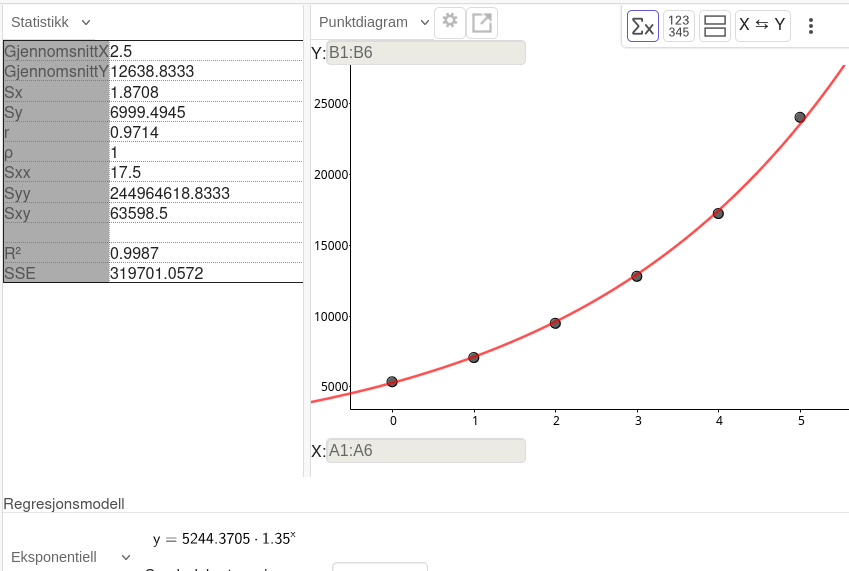
\includegraphics[scale=0.2]{opg1}
\end{figure}
\item 
\algv{
\text{Følgere i mai}=24008\cdot1,40\approx33611 \\
\text{Følgere i juni}=33611\cdot1,45\approx48736
}
\item Av siste linje i skriptet finner vi at Tuva vil få 42\% flere følgere hvis hun når målet sitt.
\pythonut{opg1.py}{
32411\; 33611\\
43755\; 48736\\
59069\; 73104\\
79743\; 113311\os

1.4209523092936056
}
}

\newpage
\subsection*{Oppgave 2}
\abc{
\item I gjennomsnitt har Solveig brukt ca. 1,5 time mer på hver tur enn Miriam. Medianene forteller at halvparten av turene til Miriam har hatt en varighet på 4 timer eller mer, mens turene til Solveig har att en varighet på 7,5 timer eller mer. At standardavviket til Miriam er større enn Solveigs betyr at det har vært større variasjon i varigheten på turene til Miraim enn på turene til Solveig.
\begin{center}
	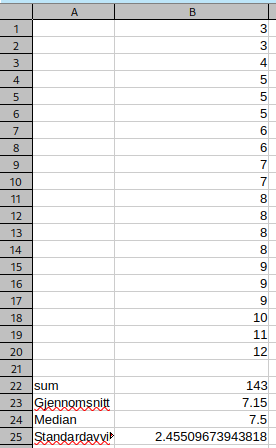
\includegraphics[scale=0.3]{opg2a}\qquad
	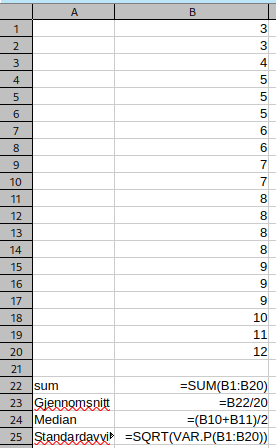
\includegraphics[scale=0.3]{opg2b}
\end{center}
\item 1) Da den kumulative frekvensen ved 3 timer er 11, mens den ved 5 timer er 14, må dette bety at de gikk 3 turer med en variget på 5 timer. \os
2) Av samme argumentering som ved 1) finner vi at de også gikk 3 turer sammen med en varighet på 8 timer. Men av de 20 turene til Solveig varte 4 av dem i 8 timer. På én av disse turene var altså ikke Miriam med.
}
\newpage
\subsection*{Oppgave 3}
Siden høyden på en søyle i et histogram er gitt som $\frac{\text{frekvens}}{\text{intervallbredde}}$, er det\\ $40\cdot 2=80$ elever på intervallet $[0, 40)$. \os

På intervallet $[0, 40)$ er det 80 elever, på intervallet $[40, 60)$ er det 120 elever, på intervallet $[60, 100)$ er det 200 elever og på intervallet $[100, 150]$ er det 100 elever. Det blir 500 elever til sammen, og da utgjør 100 elever $\frac{1}{5}$ av elevtallet. \os

Vi antar at tiden brukt fordeler seg ganske jevnt i hvert intervall. Elever i intervallet $[0, 40)$ har da i gjennomsnitt brukt 20 minutter på leksene, mens elever i intervallet $[40, 60]$ har brukt 50 minutter. Samlet tid brukt i gjennomsnitt blir da $\frac{20\cdot 80+50\cdot120}{200}=38$.\os

Da det er flere elever i intervallet $[40, 60)$ enn i intervallet $[0, 40)$, vil mediantiden for disse intervallene samlet befinne seg i intervallet $[40, 60)$. Dermed er medianen større eller lik 40, altså høyere enn gjennomsnittet på 38.

\subsection*{Oppgave 4}
\abc{
\item I begge ligningene har Sara isolert $y$ på én side, og definert de to uttrykkene som henholdsvis $f$ og $g$. I for-løkken sjekker hun om det for heltalls $x$ mellom $-4$ og $5$ er noen skjæringspunkt mellom $f$ og $g$. Skjæringspunkt er løsninger av ligningssystemet. Hun finner punkte $(-3, 0)$ og $(2, 20)$.
\item Han må skrive om funksjonene:
\[ f(x)=2x+8 \qquad,\qquad g(x)=x^2+x-48\]
I tillegg må han øke bredden på range i både negativ og positiv retning for å finne løsningene (funnet ut ved utprøving av koden). 
}

\subsection*{Oppgave 5}
\abc{
\item $r_b=\text{radius til bunn}=\frac{\text{sidelengde på kvadrat}}{2}=\frac{\sqrt{20}}{2}\approx2.2$ (rundet ned).\os
$r_t=\text{radius til topp}=\sqrt{\frac{10}{\pi}} $.\os
Figuren viser et tverrsnitt av den tenkte hele sylinderen.
Av formlikhet mellom de to grønne trekantene har vi at
$\frac{2,5}{r_b-r_t}=\frac{h_2}{r_t}$. Dermed er
\[ h_2=\frac{2,5\cdot r_t}{r_b-r_t}\approx 9.87 \]
\begin{figure}
	\centering
	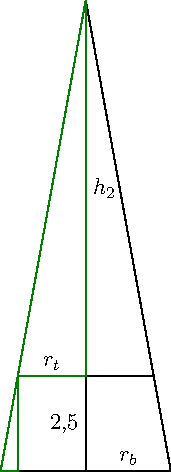
\includegraphics[]{opg5}
\end{figure}

Altså er $\text{høyden til hele sylinderen}\approx 12,37$.
\item \alg{
&\text{volum til øverste sylinder}\approx \frac{10\cdot 9,87}{3}=33 \os
&\text{volum til nederste sylinder}\approx \frac{\pi\cdot2.2^2\cdot12.37}{3} \approx 63\os
&\text{volum til vegg}\approx 63-33=30
}
$30\enh{m}^3$ tilsvarer 30\,000 liter.
}

\newpage
\subsection*{Oppgave 6}
\abc{
\item Siden lånekostnaden er oppgitt som en fast utgift per måned kan man gå ut i fra at det er et annuitetslån. Lånet krever 15\% egenkapital. 15\% av 2\,000\,000 er lik 300\,000, og da er det 1\,700\,000\enh{kr} som må lånes.
\item Hvis den månedlige renten er 1,5\%, vil beløpet ganges med 1,015 hver måned. Etter et år vil dette tilsvare å gange startbeløpet med $1,015^{12}$.\os

Vi setter vekstfaktoren ved en månedlig rente lik $x$. Ved en årlig rente lik 5,49\% er da
\alg{
x^{12} &= 1,0549 \\
x &= \sqrt[12]{1,0549} \\
&\approx 1,0045
}
Dette tilsvarer en månedlig rente lik 0,45\%.
\item Terminbeløpet i et annuitetslån er summen av rentene og avdraget. Med en månedlig rente lik 0,47\% er det første rentebeløpet lik $1\,700\,000\cdot0,0045=7650$.
Altså er det 7\,650\enh{kr} i renter og $10\,495\enh{kr}-9\,400\enh{kr}=2\,845\enh{kr}$ i avdrag. Dette betyr at rentene utgjør ca. 75\% av termingebyret, og avdraget ca 25\%.
\item For å undersøke om Johannes har råd til lånet, må vi ta med vilkåret om at lånet skal kunne betales selv ved en renteøkning på 3 prosentpoeng. Ved samme utrekning som i b) finner vi at i så fall er den månedlige renten lik 0,68\%. Det er ganske omfattende å regne ut eksakt hva det nye terminbeløpet vil bli med denne renten, derfor gjør vi denne forenklingen: Vi regner at den prosentvise økningen i månedlig rente tilsvarer den prosentvise økningen av terminbeløpet. Da er
\[ \text{nytt terminbeløp}=\frac{0,68}{0,45}\cdot10\,495\enh{kr}\approx 15\,589\enh{kr}\]
\newpage
Av differansen funnet i regnearket ser vi at Johannes har råd til lånet både ved og uten en renteøkning.
\begin{figure}
	\centering
	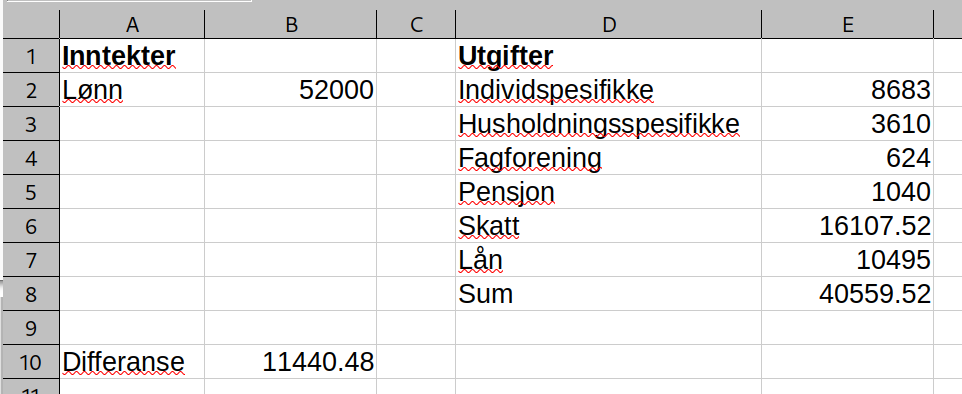
\includegraphics[scale=0.2]{opg6a}\qquad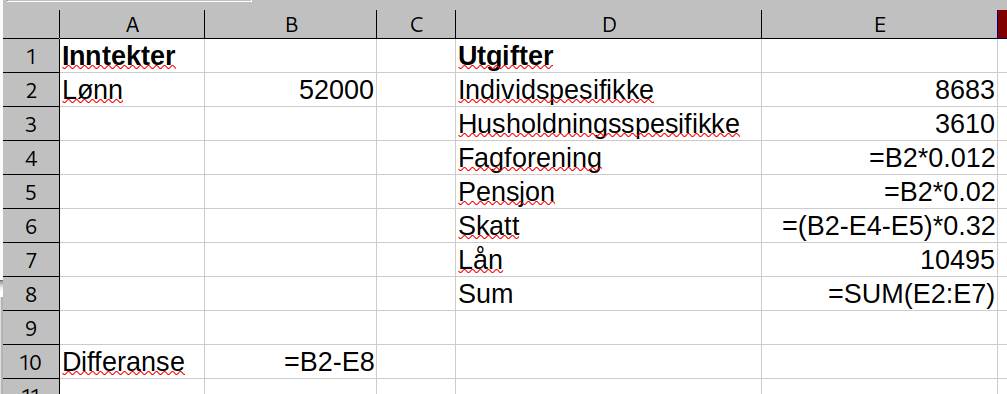
\includegraphics[scale=0.2]{opg6b}
\end{figure}
}



\end{document}